\documentclass{article}
\usepackage[utf8]{inputenc}

\usepackage{graphicx}

%\usepackage[english]{babel}
%\usepackage{biblatex}

\PassOptionsToPackage{hyphens}{url}\usepackage{hyperref}
\begin{document}
\begin{titlepage}
	\centering
	{\scshape\LARGE Sussex University \par}
	\vspace{1cm}
	{\scshape\Large Final year project\par}
	\vspace{1.5cm}
	{\huge\bfseries FYP-DHT\par}
	\vspace{2cm}
	{\Large\scshape Michael Sledge\par}
	{\Large CN:121677\par}
	\vspace{1cm}
	{\Large Computer Science MComp\par}
	{\Large\itshape Department of Informatics\par}
	\vspace{1cm}
	supervised by\par
	George Parisis

	\vfill

% Bottom of the page
	{\large 2016\par}
\end{titlepage}

\section{Statement of Originality}
This report is submitted as part requirement for the degree of Computer Science at the University of Sussex. It is the product of my own labour except where indicated in the text. The report may be freely copied and distributed provided the source is acknowledged.
\newpage

\section{Summary}


\newpage
\tableofcontents
\newpage


\section{Introduction}

%this should give the motivation for the project. The aims of the project should at least be stated in the first paragraph, but preferably in the first sentence.

to build a system for creating distributed computing applications more easily by implementing a consistent means of organising computing nodes and enabling communication between them without each node's applications needing knowledge of the other nodes in the system.


%


% explain the structure of the report.
This report will cover professional and ethical considerations, related research and systems, more detailed technical requirements, and a record of phases which have been completed and those still to be completed.

\subsection{Professional Considerations}
The BCS Code of Conduct \cite{bcscoc} sets out the following standards which may be relevant to this project: 2 c) “develop your professional knowledge, skills and competence on a continuing basis, maintaining awareness of technological developments, procedures, and standards that are relevant to your field.” and 2 d) “ensure that you have the knowledge and understanding of Legislation* and that you comply with such Legislation, in carrying out your professional responsibilities.”

From ‘Professional Competence and Integrity’ in Annex A Interpretation of the BCS Code of Conduct \cite{bcscoca}: “You should seek out and observe good practice exemplified by rules, standards, conventions or protocols that are relevant in your area of specialism.”

Existing libraries may be used in this project and their licenses must be followed, standards and conventions in languages used should be followed also.



%\section{REPORT BODY}

\section{Background Reading/Existing solutions}
The chord protocol \cite{chord} uses consistent hashing to assign keys to nodes. It defines a set of functions which nodes use to build and maintain a chord network. Chord nodes in a network form a virtual ring in which each node is aware of its immediately adjacent nodes as well as several succeeding nodes.
Nodes are mapped into the same keyspace used for identifiers for the application
Each node knows how to find the node that an identifier maps to, illustrated in fig 1. If the id is between the current node and its successor then it maps to the successor, otherwise it asks the furthest node it knows about that is not past the id in the keyspace. The succeeding nodes that a node has knowledge of are stored in a 'finger' table (illustrated as dashed arrows in fig 1.) These are not necessary for functionality but they reduce the number of steps when mapping a key to a node.
\begin{figure}
\centering
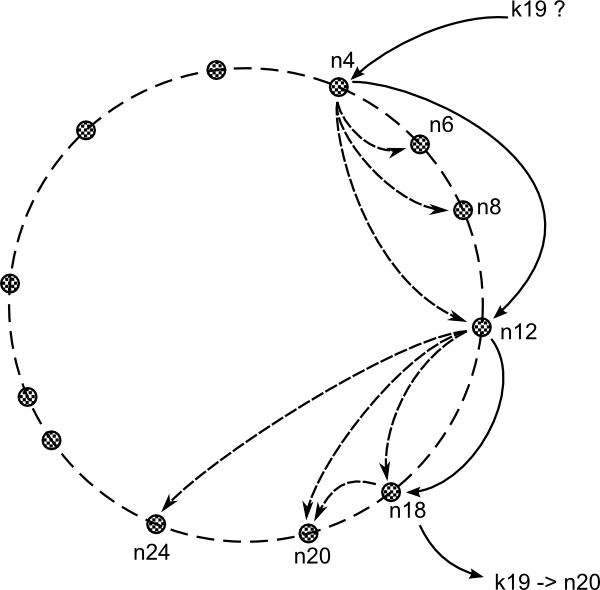
\includegraphics{chord_find-successor.png}
\caption{Finding the successor for key 19. Dashed arrows show which nodes a node has knowledge of (some have been omitted for clarity).}
\end{figure}

The stabilisation that chord nodes run periodically is important to keep the network functional as the availability of nodes changes. Stabilisation is executed as follows: the node checks if there is a node between itself and its recorded successor, if there is it updates its recorded successor; then the node notifies its recorded successor of its existence so it can update its predecessor record if necessary. Nodes also periodically update their finger tables, and check whether their predecessor is still accessible.
\begin{figure}
\centering
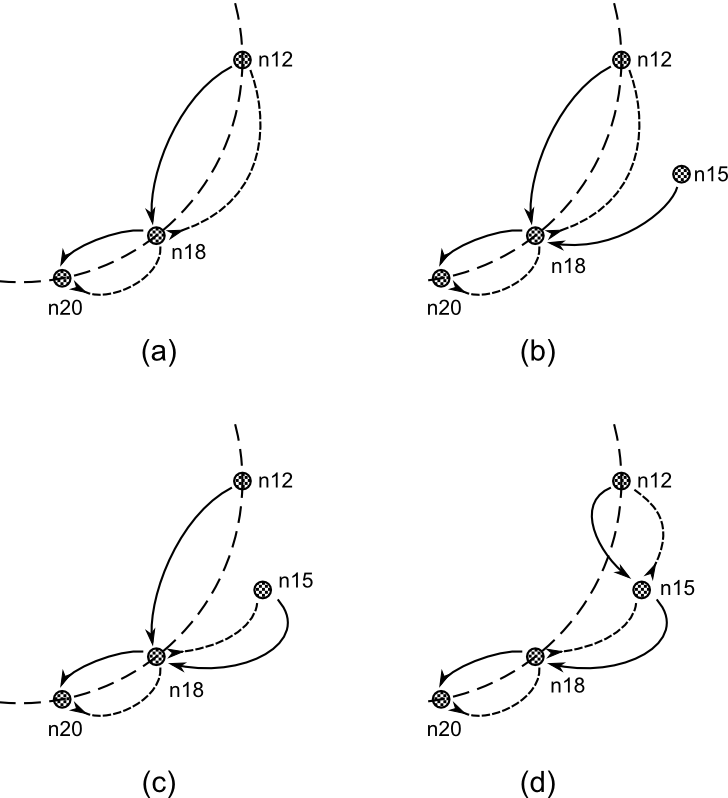
\includegraphics{chord_joining.png}
\caption{Node joining and stabilisation. (a) A chord network in a stable state. (b) new node n15 joins having found its successor (c) n15 runs its stabilisation and now n18 is aware of n15. (d) n12 runs its stabilisation and the network is back to as stable state}
\end{figure}
\\
\\
Memcached [4] is a distributed in-memory caching system based on a distributed hash table intended for use in speeding up web applications by caching database entries, though it is possible to use it for other similar purposes. It is used by many large web companies.

Memcached uses spare memory on web servers to create a distributed in-memory cache which can be used to alleviate server load. This provides several benefits when compared to having each server managing it's own individual cache: the combined cache is much larger than individual caches; cached data is consistent any server requesting the a key in the cache will get the same value, whereas separate caches may not update data at the same time; improved scalability, as more servers are added to handle increasing load the size of the cache increases, making large scaling much easier than it would be with individual caches per server.
\\
\\
Mace [5] is a toolkit for building distributed systems which “seeks to transform the way distributed systems are built by providing designers with a simple method for writing complex but correct and efficient implementations of distributed systems.” [6] It is designed to provide a common 'language' to design distributed systems without having to implement the entire system from scratch, it provides and uses libraries to build systems. The restrictions mace imposes in this way allow for better options for debugging a distributed system.

Nodes in mace are made up of one or more layers and each layer is built on an event driven state machine. Like Chord, Mace creates a virtual overlay network in which each node keeps a record of adjacent nodes, periodically updating these records and notifying the application when changes occur.
\\
\\
Libevent [7] is a cross platform C library which provides a single API for implementing event driven network servers using one of a number of mechanisms systems provide for event notification, to allow for asynchronous I/O operations. Libevent checks for events and runs the callbacks specified for each event in the queue. An event can be a notification for a socket becoming read- or write-able, a new connection on a listen socket or a timer event among other things. Libevent also provides bufferevents to simplify the task of using read and write buffers with socket events. Libevent also includes a simple HTTP, DNS and RPC (remote procedure call) implementations.
\\
\\
Similar to Libevent, Boost.Asio [8] is a cross platform C++ library providing a consistent API for network and low level I/O programming with an asynchronous model. Its scope is slightly narrower than libevent's, so it doesn't include the simple protocol implementations.




\section{Requirements Analysis}
Build a high performance library for building DHT based systems with asynchronous I/O for scalability. Nodes should be independent and self organising, requiring no central authority, and be tolerant of joining, leaving and failing of nodes in the system.

\subsection{Functional requirements}
\begin{itemize}
\item
Creating and joining a network
\item
Finding the node a key maps to from any node on the network.
The algorithm finds the node a key maps to directly or finds the next hop and passes the job of finding it on to that node.
\item
Periodic stabilisation to account for change in availability of nodes.
Periodic checking for failures of adjacent nodes and arrival of new nodes. New nodes must notify at least one node of their presence.
\item
Allow sending of messages or data to other nodes for the application.
Once the node a key maps to has been found allow data to be sent to that node.
\item
Provide callbacks for the application when a message is received.
Allow the application programmer to provide functions which are called when specific events occur.
\item
Provide callbacks for notifying the application of changes in the availability of nodes that may affect it, i.e. the next and previous nodes. Specifically when the set of keys a node is responsible for changes.
\end{itemize}


\subsection{Non-functional requirements}
\begin{itemize}
\item
Provide high performance network communication between nodes
\item
Be highly scalable both in terms of number of nodes and the load of individual nodes assuming the application is able to handle such loads.
\end{itemize}

\section{Design and Building}

\subsection{Design Process}

The design involves multiple modules or layers

\subsection{Design Principals}
Several design principals were

\subparagraph{No global state}
This makes it easier to create thread-safe code and allow multiple instances to be instantiated within a single process. It allows for a more functional approach wherein all state has to be passed to functions as a arguments, this will mean that they can be implemented so to, as far as possible, always behave consistently way when given the same input.

\subparagraph{Layered structure}
Organising a large amount of code can be
The code will be organised into separate layers which utilise the layers below them but do not assume knowledge of layers above. this minimises interdependencies between modules.

\subparagraph{Defensive programming}
check all function input to prevent errors like segfaults

\subsection{Design Details}

\paragraph{The Network layer}
The network layer handles open connections as well as the listen socket. It mostly acts as a wrapper for libevent and provides a simplified interface for the layers above. The main data structure is \texttt{struct net\_server} which is an instance of the net layer which needs to be passed to the majority of functions. It holds references to an event base (libevent's main data structure); open connections; and the listen socket. The layer contains functions for creating, activating and configuring connections.
\subparagraph{Usage}
Initialise a new server instance by providing a listen port number and a callback function and argument for accepting incoming connections. Once any other setup is complete, the function \texttt{net\_server\_run} can be called which starts the event loop and does not return until the loop exits and as such users must start another thread if they wish for their application to do more than wait for incoming connections.
\\
On receiving notification of an accepted connection (via callback), the application should set read, error/disconnect, and optionally write handlers for the newly accepted connection.
\\
Users can create outgoing connections by providing a remote IP and port this sets up the connection internally but does not activate it, this allows the user to add data to the write buffer before connecting if desired.
\\
Both accepted incoming and outgoing connections use the same interface, allowing setting of callback functions for read, write and other events; setting of the callbacks' custom argument; getting the connection's read and write buffers; setting the connection's timeouts; getting the remote address (useful for some types of messages on incoming connections); and getting the underlying buffer event for finer control

\subparagraph{Internals}
The net server keeps a list of references to open connections and keeps track of the callbacks that have been set for each one. It also has a mutex lock for the connection list to prevent concurrent modification as it is likely that the event loop thread may accept a connection while another thread requests creation of an outgoing connection.
\\
Connections use libevent's \texttt{buffer\_event} which can be used to automatically read incoming data from a socket to a buffer and write data to a socket from a buffer as the socket becomes readable and writeable respectively, they can be set to invoke there callbacks when the buffers contain more or less than a given amount of data.

\paragraph{The Node layer}
The node layer is the main body and contains code for creating, joining and maintaining the network of nodes and routing, these are together due to the fact that joining and maintaining the network requires routing messages between nodes. Much like the net layer its main data type is a handle to a node instance, the interface similarly consists of a function to initialise a new node instance and functions to join an existing network or create a new one. 
\subparagraph{Usage}

\subparagraph{Internals}
A node instance contains a reference to its own net server instance.
The node layer can be split into a few sub modules: Handling incomming messages from other nodes; network maintenance; message routing; initiating communications with other nodes

\paragraph{Communication Protocol}
Messages sent between nodes use a TLV (type-length-value) format, in other words they consist of a header, containing a single byte indicating the type of message and a 4 byte value indicating the length of the body, and the body itself which contains the actual information formatted according to the message type

\subsection{Example applications}

\paragraph{1. textsend}

\section{Testing}

\section{Evaluation}

\section{Conclusion}

\section{References}

\bibliographystyle{plain}
\bibliography{report}

% \printbibliography

%\section{Appendices}

\section{Appendices}
\appendix
\section{Message protocol}

Messages are made up of a single bit defining the type of the message; a 4 byte value for the length of the message body; and the optional, variable length message body.

\subsection{Type bit values}
\begin{tabular}{|l | l|}
\hline
\texttt{'S'} & Ask node for successor of id \\\hline
\texttt{'s'} & Return successor of id \\\hline
\texttt{'P'} & Ask a node for its predecessor \\\hline
\texttt{'p'} & Returning a node's predecessor \\\hline
\texttt{'N'} & Notify another node that the sender believes it is that node's predecessor \\\hline
\texttt{'n'} & Reply acknowledging predecessor notification \\\hline
\texttt{'A'} & Used to check the availability of a node\\\hline
\texttt{'a'} & Reply to confirm that a node is operating \\\hline
\texttt{'M'} & The contents of the message is for the application using the library \\\hline
\texttt{'0'} & Signifies Unknown message type \\\hline
\end{tabular}

\subsection{Body Layouts}







\end{document}